\section{Evaluation}
To answer the initial question "How suitable are beacons for mobility studies?" we evaluated the technology based on different criteria.

\subsection{Evaluation of Beacons for Mobility Studies}

\begin{itemize}
\item Cost and effort: 
\par Beacons are inexpensive and easy to deploy. Therefore, they are well suited for fast and large distribution.
\item Accuracy:
\par To attain a perfect level of accuracy for a mobility study beacons would have to detect every single device that is passing by. The device would need to be identified uniquely, so the researcher can anticipate the movement of a single device. In our field study only approximately 4\% of the passing devices where detected. We also cannot say with high certainty if a device that was detected is the same that has been detected by a different beacon. Therefore the accuracy of beacons is too low to use them in a mobility study.
\item Granularity:
\par We do not have any additional information about the owner of a detected device, so no granularity of different student groups can be detected.
\item Privacy: 
\par No personal data is connected to the beacon detection the privacy is protected.
\item Value:
\par If the beacons were working 100\% as intended they would offer high value information for a mobility study. One could tell when how many devices are in what place at what time. One could also tell the movement behavior of different devices, if they could be identified uniquely. 
\item unobtrusiveness: 
\par In the use of a mobility study they are unobtrusive because the students devices interact with the beacons without anything noticed by the student. 
\end{itemize}

The status quo still has to many problems that can yet not be overcome to make beacons a feasible technology for mobility studies. In future scenarios this might change. The results from the simulation give some insights into possible scenarios. 

\subsection{Simulation Results}

Based on the given data described in chapter 4.5 Student Mobility Simulation section a scenario was created that replicates the current situation. Where no data was available reasonable assumptions for variables were made.
Going from this as a base line two future scenarios were created, that simulate a near future in 3-5 years: (1) an average case scenario and (2) a best case scenario (cf. Table \ref{table:simulation}).

\begin{table}[htbp]\centering
\caption{Simulated Scenarios about Beacon Detection}
\footnotesize {Three scenarios were simulated: (1) The current scenario, as the situation is today, (2) an average case future scenario, (3) a best case future scenario}
\label{table:simulation}
\end {table}
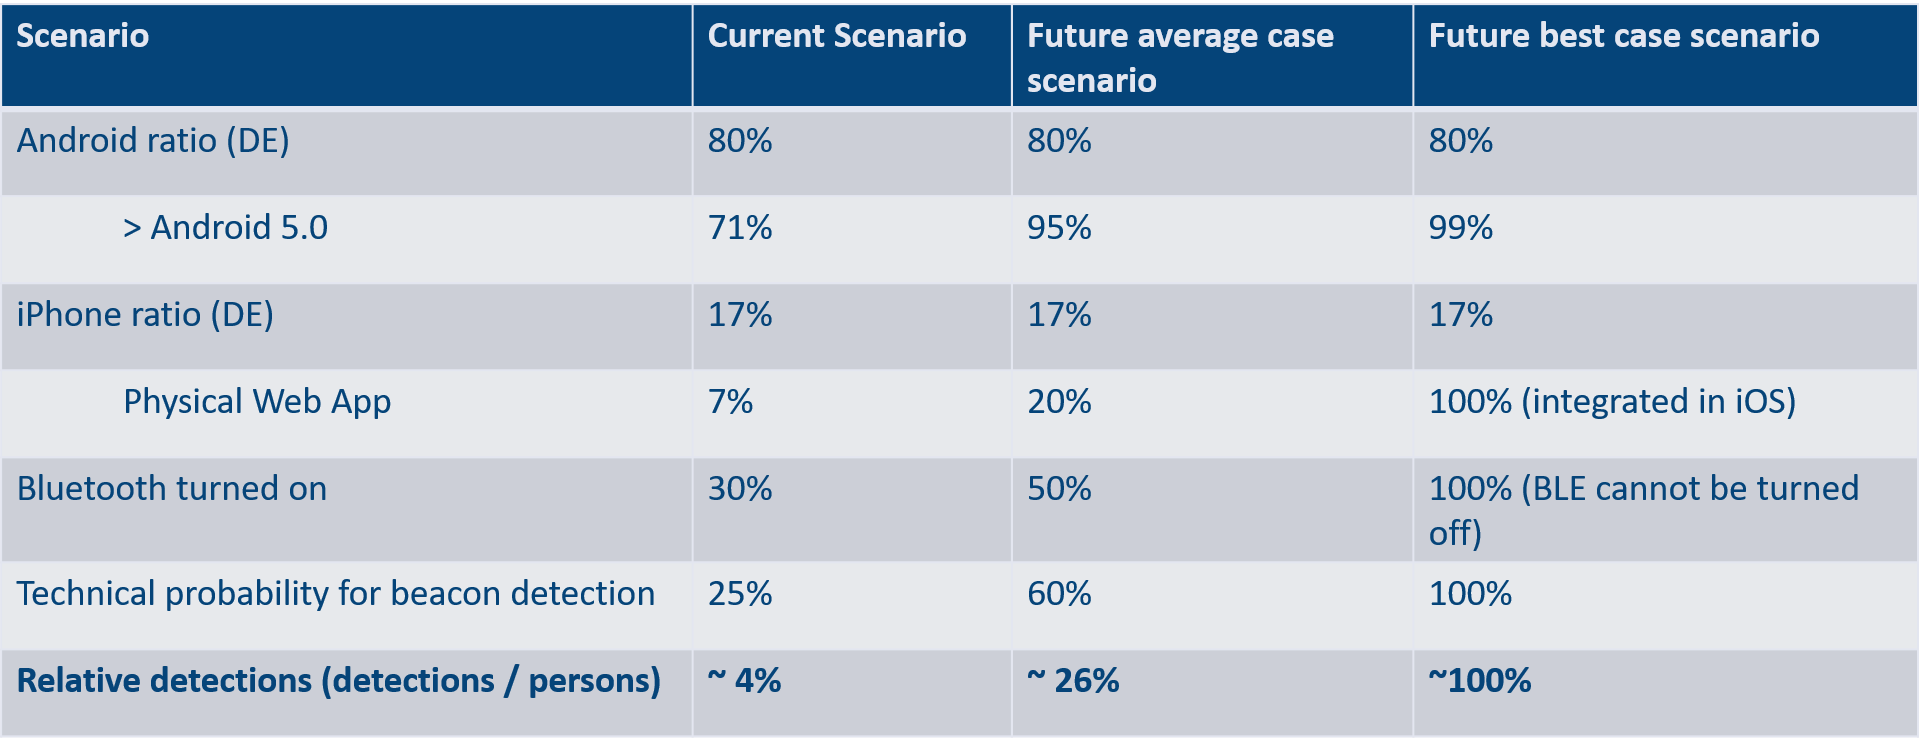
\includegraphics[height=50mm]{evaluation/images/table_simulation}
	
\paragraph{Current Scenario}

The current scenario tries to reproduce the status as it is today as good as possible. 

The current scenario used the following values:
\begin{itemize}
\item Android ratio in Germany: 80\%
\item Percentage of Android devices with Android version > 5.0: 71\%
\item iPhone ratio in Germany: 17\%
\item iPhones with Physical Web App installed: 7\%
\item Bluetooth turned on: 30\%
\item Technical probability for beacon detection: 25\%
\end{itemize}

After running the simulation this results in a detection rate - devices detecting beacons divided by devices that passed by the beacons - of 4\%. This detection rate matches our experiences with the beacons that we places within the ERBA building. According to the cafeteria staff 400 to 700 people are in the cafeteria throughout the entire day. With an average detection of 20 devices per day in the cafeteria we get a rough estimation of 4\% detection rate, which matches our simulation.
\par The parameters for the interactions were set according to our experiences with the distributed beacons: Within lecture halls an interaction rate of about 7\% and within the cafeteria an interaction rate of about 1.5\%. We did not distribute any beacons within foyers or entrances, but we assumed an interaction rate of 0.1\% for people only walking by a beacon and not dwelling within the room.


\paragraph{Future Average Case Scenario}

From our current scenario we can now vary different factors and observe how the detection rate changes. We cannot say for sure how those variable will change in the future, but we can make reasonable assumptions.
\par For the average case scenario we assumed that more Android users will have a higher operation system and more people will have Bluetooth turned on (cf. chapter 4.5 Student Mobility Simulation). 
Due to technical improvement the technical probability for beacon detection is assumed to have risen. 

The future average case scenario used the following values:
\begin{itemize}
\item Android ratio in Germany: 80\%
\item Percentage of Android devices with Android version > 5.0: 95\%
\item iPhone ratio in Germany: 17\%
\item iPhones with Physical Web App installed: 20\%
\item Bluetooth turned on: 50\%
\item Technical probability for beacon detection: 60\%
\end{itemize}

This results in a detection rate of 26\%. We assume this to be a reasonable value that can be reached within the next few years.

\paragraph{Future Best Case Scenario}

For the best case scenario we assume that all parameters are turning out in the best possible way for beacon detection. This includes, that the iOS of iPhones will have a similar function as the Android Nearby included, that will be distributed with a new iOS to all iPhone devices. 
\par Also, the assumption is made that for future smartphones it will not be possible to turn off the Bluetooth Low Energy anymore, and therefore smartphones can always receive beacon signals. Of course, this change of hardware will not take place within the next few years because unlike the iOS it cannot be distributed to all devices at once. It relies on the customers switching from an old smartphone to a newer one.
\par This scenario also assumes, that all technical problems with the beacon detection are eliminated and every beacon that should be detected by a smartphone, will be detected.


The future average case scenario used the following values:
\begin{itemize}
\item Android ratio in Germany: 80\%
\item Percentage of Android devices with Android version > 5.0: 99\%
\item iPhone ratio in Germany: 17\%
\item iPhones with Physical Web App installed: 100\%
\item Bluetooth turned on: 100\%
\item Technical probability for beacon detection: 100\%
\end{itemize}

As all values in favor of beacons are set to 100\% this results in a detection rate of 100\%. This scenario is not likely to happen within the next 3 to 5 years. Maybe within a more distant future this is a possibility.
